\providecommand{\mainpath}{..} % Command to retrieve the path of the main file. It must be defined before documentclass.

\documentclass[\mainpath/main]{subfiles}
\begin{document}

\chapter{User Interfaces Design}
\label{UIDesign}

% Command to be executed after the starting of every chapter
\setmyfancystyle
% ----------------

In this chapter are shown the main \glspl{mockup} of myTaxiService, due to present the graphical user interfaces of the system for each functionality. All the \glspl{mockup} are displayed with an accurate description to prevent misunderstanding and to recall the functionality.\\

\section{Registration/Login}
When an user connects to the WS or opens the MA, the first screens is the login page. For both the versions, there is a button to redirect to the registration page, if the user is not registered yet.\\
The figure \ref{UI:loginWS} is the WS version where the registration button is made by a link on the phrase \textquotedblleft Not Registered yet? Click here\textquotedblright. At the same time the user can insert his credentials into the specific boxes.\\
The figure \ref{UI:loginMA} is the corresponding \gls{mockup} for the mobile application: at the application opening the user can inserts his credentials or clicks on the registration button.\\

\clearpage

\begin{figure}[ht!]
	\centering
	\begin{minipage}[t]{0.45\textwidth}
		\centering
		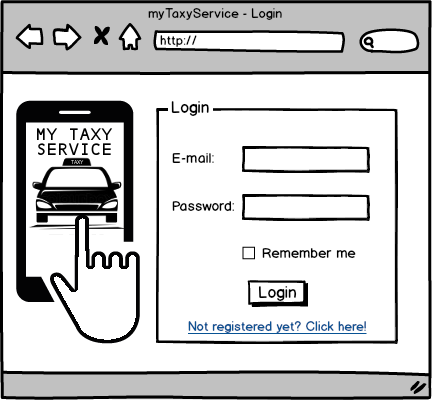
\includegraphics[width = \linewidth] {mockups/Login_WS}
		\caption{Login page into website.}
		\label{UI:loginWS}
	\end{minipage}
	\hspace{0.05 cm}
	\begin{minipage}[t]{0.45\linewidth}
		\centering
		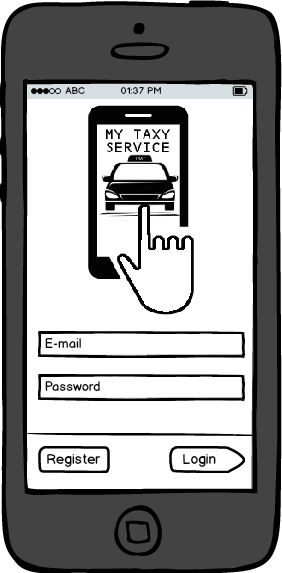
\includegraphics[height = 8cm] {mockups/Login_MA}
		\caption[Login page into mobile application.] {\scriptsize Login page into mobile application.}
		\label{UI:loginMA}
	\end{minipage}
\end{figure}

A non registered user has to enrol into the system, so he clicks on the corresponding button and he is redirected to that page. The figures \ref{UI:registrationWS} and \ref{UI:registrationMA} shows the \glspl{mockup} for this: into the \gls{ma} the box labels are written into them and disappears when the user fills in; into the \gls{ws} the labels are shown near the corresponding one.\\

\begin{figure}[ht!]
	\centering
	\begin{minipage}[t]{0.45\textwidth}
		\centering
		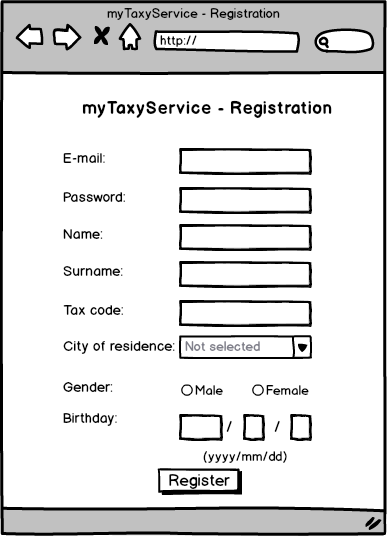
\includegraphics[width = \linewidth] {mockups/Registration_WS}
		\caption{Registration page into website.}
		\label{UI:registrationWS}
	\end{minipage}
	\hspace{0.05 cm}
	\begin{minipage}[t]{0.45\linewidth}
		\centering
		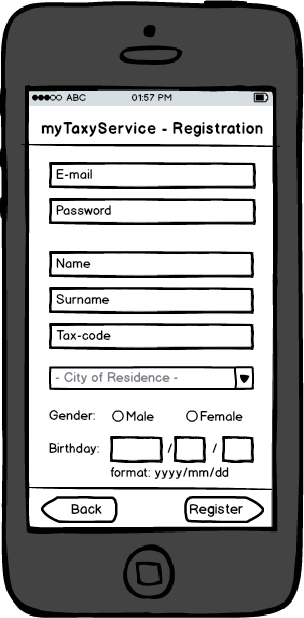
\includegraphics[height = 8cm] {mockups/Registration_MA}
		\caption[Registration page in mobile application.] {\scriptsize Registration page in mobile application.}
		\label{UI:registrationMA}
	\end{minipage}
\end{figure}

\section{Personal Information Management}
The figures \ref{UI:managePersonalInformationWS} and \ref{UI:rmanagePersonalInformationMA} show the mockups for the  management of personal information.\\
The only information that can be modified are the email, the password and the city of residence. In both the myTaxiService's versions the other information are shown into a non-modifiable boxes (so they have a different color, typically grey, to mark this property).

\begin{figure}[ht!]
	\centering
	\begin{minipage}[t]{0.45\textwidth}
		\centering
		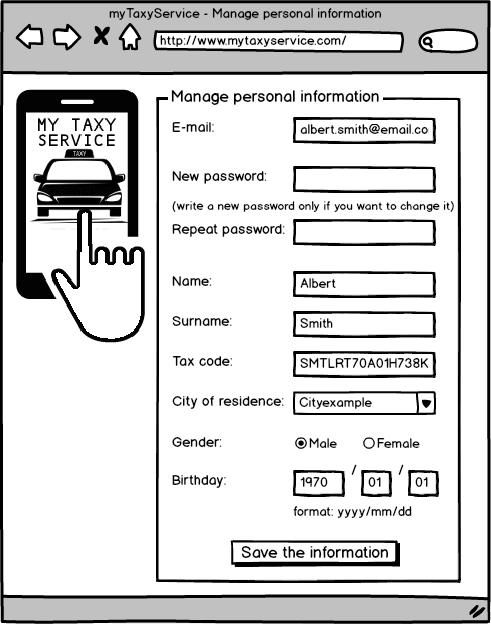
\includegraphics[width = \linewidth] {mockups/ManagePersonalInformation_WS}
		\caption{Personal Information Management page into website.}
		\label{UI:managePersonalInformationWS}
	\end{minipage}
	\hspace{0.05 cm}
	\begin{minipage}[t]{0.45\linewidth}
		\centering
		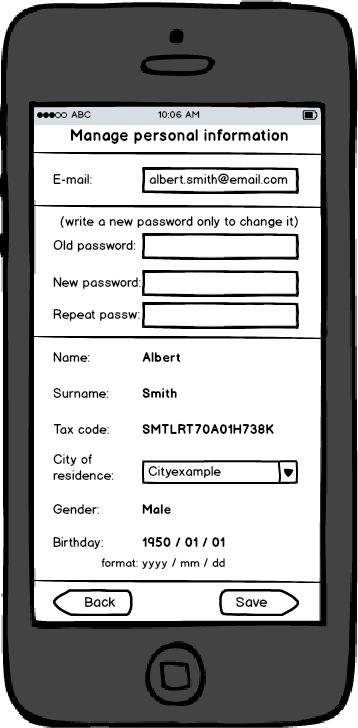
\includegraphics[height = 9cm] {mockups/ManagePersonalInformation_MA}
		\caption{Personal Information Management page in mobile application.}
		\label{UI:rmanagePersonalInformationMA}
	\end{minipage}
\end{figure}

\clearpage

\section{Driver functionalities}
The functionalities reserved for the cabmen are developed only for the \gls{ma} version of myTaxiService: the reasons are explained in \autoref{ArchitecturalDesign:preamble}. When a cabman has to notifies the system that it is starting his workshift or he has ended a ride, so he is now waiting for a new ride, he uses the Start Waiting Time functionality that is shown in figure \ref{UI:startWaitingTime}: the displayed position is calculated by GPS.\\

\begin{figure}[ht!]
	\centering
	\begin{minipage}[t]{0.45\textwidth}
		\centering
		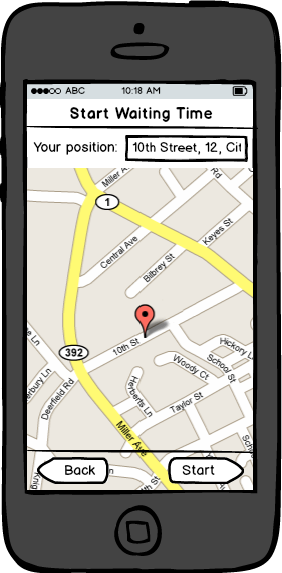
\includegraphics[height = 9 cm]{mockups/StartWaitingTime}
		\caption{The Start Waiting Time page.}
		\label{UI:startWaitingTime}
	\end{minipage}
	\hspace{0.05 cm}
	\begin{minipage}[t]{0.45\linewidth}
		\centering
		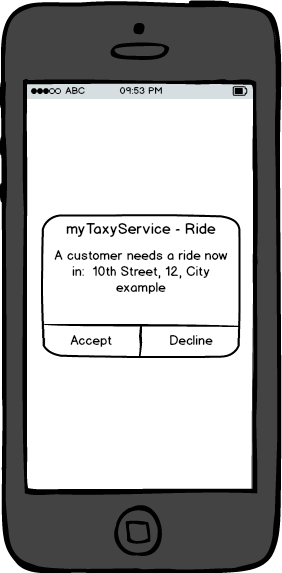
\includegraphics[height = 9 cm]{mockups/AcceptDenyRide}
		\caption[The request for a ride to a driver page.]{The request for a ride page.}
		\label{UI:acceptDenyRide}
	\end{minipage}
\end{figure}

During this period, the system can asks the driver to make a ride, so in figure \ref{UI:acceptDenyRide} it is shown the screen for this request.\\
At last, in figure \ref{UI:workshift} there is a mockup for the page where the driver can modify his workshifts. He can add, modify or remove them. The page where the driver can see his workshifts is not displayed, but it is similar to the shown one, without the modification symbols.\\
\\
\\

\begin{figure}[ht!]
	\centering
	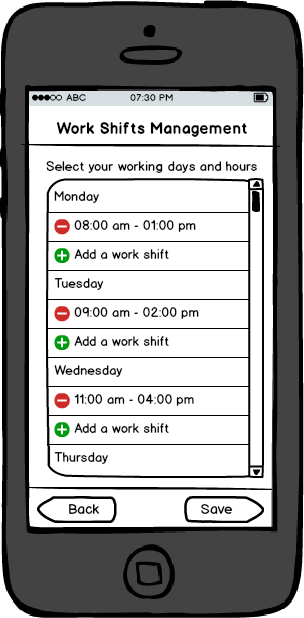
\includegraphics[height = 8 cm]{mockups/WorkShiftsManagement}
	\caption{The workshifts management page.}
	\label{UI:workshift}
\end{figure}

\section{Zerotime Ride}
When a user asks for a zerotime ride, he has to insert the starting and the destination positions (the first one can be calculated by the GPS) and then to confirm the request.\\
In the \gls{ma} this sequence of operations is performed with three screens (mockups in figures \ref{UI:zerotimeMA1}, \ref{UI:zerotimeMA2} and \ref{UI:zerotimeMA3}), while into the \gls{ws} it is used only one screen split into the correspondent sections, shown in figure \ref{UI:zerotimeWS}.

\begin{figure}[ht!]
	\centering
	\begin{minipage}[t]{0.4\textwidth}
		\centering
		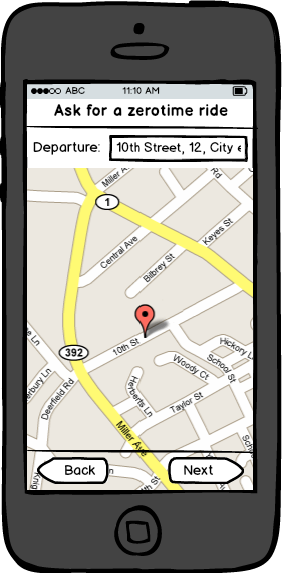
\includegraphics[height = 8 cm]{mockups/AskForZerotimeRide_MA_1}
		\caption[Zerotime ride request part1 into mobile application.]{Zerotime ride request into mobile application: starting position insert (manually or by GPS) page.}
		\label{UI:zerotimeMA1}
	\end{minipage}
	\hspace{1 cm}
	\begin{minipage}[t]{0.40\linewidth}
		\centering
		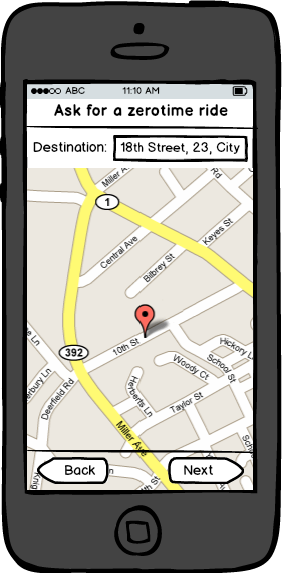
\includegraphics[height = 8 cm]{mockups/AskForZerotimeRide_MA_2}
		\caption[Zerotime ride request part2 into mobile application.]{Zerotime ride request into mobile application: destination position insert page.}
		\label{UI:zerotimeMA2}
	\end{minipage}
\end{figure}

\begin{figure}[ht!]
	\centering
	\begin{minipage}[t]{0.4\textwidth}
		\centering
		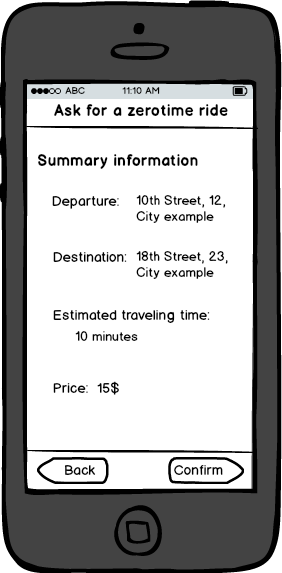
\includegraphics[height = 8.5 cm]{mockups/AskForZerotimeRide_MA_3}
		\caption[Zerotime ride request part3 into mobile application.]{Zerotime ride request into mobile application: confirmation page.}
		\label{UI:zerotimeMA3}
	\end{minipage}
	\hspace{1 cm}
	\begin{minipage}[t]{0.40\linewidth}
		\centering
		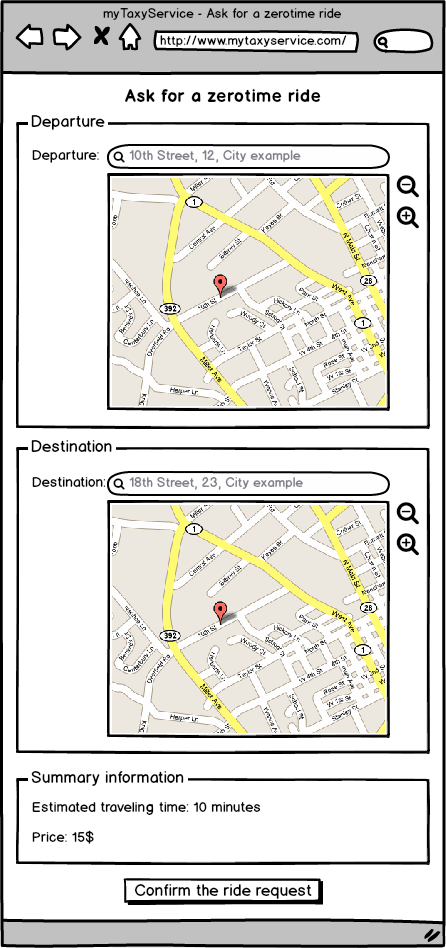
\includegraphics[height = 8.5 cm]{mockups/AskForZerotimeRide_WS}
		\caption[Zerotime ride request into website.]{Zerotime ride request into website page.}
		\label{UI:zerotimeWS}
	\end{minipage}
\end{figure}

\clearpage

\section{Future Ride}
When a user desires to book a future ride, he has to insert the starting and the destination positions (the first one can be calculated by the GPS), the departure (both the date and the time) and then to confirm the request.\\
In the \gls{ma} this sequence of operations is performed with three screens (mockups in figures \ref{UI:futuretimeMA1}, \ref{UI:futuretimeMA2} and \ref{UI:futuretimeMA3}), while into the \gls{ws} it is used only one screen split into the correspondent sections, shown in figure \ref{UI:futuretimeWS}.\\
In both the \gls{ma} and the \gls{ws}, the departure inserting is made with a popup that uses the apposite operative system functionalities to insert the dates (for example a computer OS can use a calendar for dates and a box for time, while a mobile OS can use a dropdown list or something that slides following the finger's touch).\\

\begin{figure}[ht!]
	\centering
	\begin{minipage}[t]{0.4\textwidth}
		\centering
		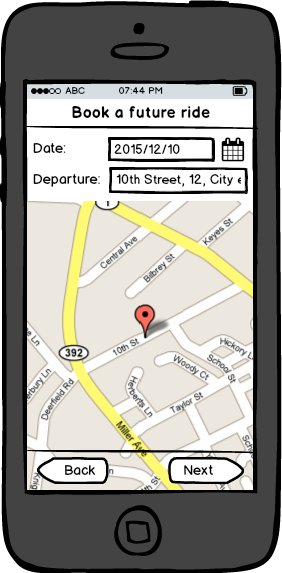
\includegraphics[height = 9 cm]{mockups/BookFutureRide_MA_1}
		\caption[Future ride request part1 into mobile application.]{Future ride request into mobile application: departure starting position insert (manually or by GPS) page.}
		\label{UI:futuretimeMA1}
	\end{minipage}
	\hspace{1 cm}
	\begin{minipage}[t]{0.40\linewidth}
		\centering
		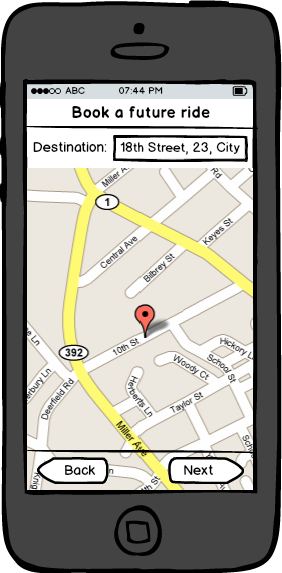
\includegraphics[height = 9 cm]{mockups/BookFutureRide_MA_2}
		\caption[Future ride request part2 into mobile application.]{Future ride request into mobile application: destination position insert page.}
		\label{UI:futuretimeMA2}
	\end{minipage}
\end{figure}

\begin{figure}[ht!]
	\centering
	\begin{minipage}[t]{0.4\textwidth}
		\centering
		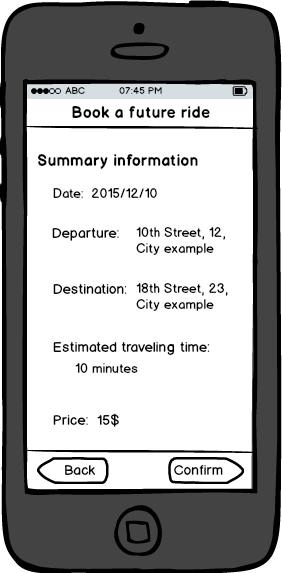
\includegraphics[height = 9 cm]{mockups/BookFutureRide_MA_3}
		\caption[Future ride request part3 into mobile application.]{Future ride request into mobile application: confirmation page.}
		\label{UI:futuretimeMA3}
	\end{minipage}
	\hspace{1 cm}
	\begin{minipage}[t]{0.40\linewidth}
		\centering
		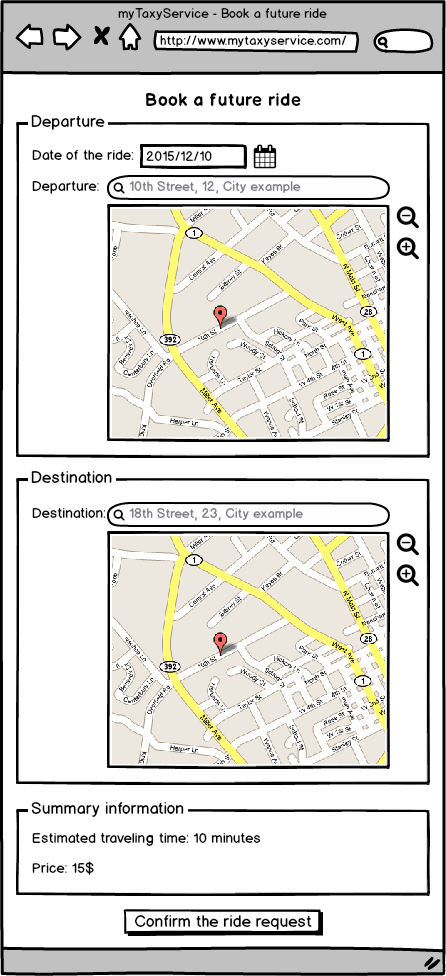
\includegraphics[height = 9 cm]{mockups/BookFutureRide_WS}
		\caption[Future ride request into website.]{Future ride request into website page.}
		\label{UI:futuretimeWS}
	\end{minipage}
\end{figure}

\section{Other User Functionalities}
myTaxiService gives other useful functionalities to the users.\\
In \gls{ma} there are two screens: in figure \ref{UI:reservationMA1} the users can see all his reservation split into two sections, one for the future reservation (they can be edited) and one, at the bottom, for a list of the past rides; in figure \ref{UI:reservationMA2} the user can edit a specific reservation (either the departure or the positions can be modified) that it was selected in the previous page by a click on the \textquotedblleft edit, delete\textquotedblright  button.\\

\clearpage

\begin{figure}[ht!]
	\centering
	\begin{minipage}[t]{0.4\textwidth}
		\centering
		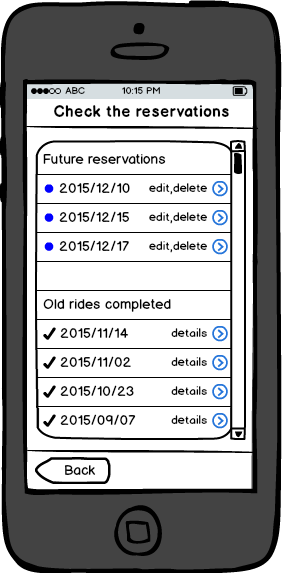
\includegraphics[height = 8 cm]{mockups/CheckReservations_MA_1}
		\caption[View reservation into mobile application.]{The view reservations page into mobile application.}
		\label{UI:reservationMA1}
	\end{minipage}
	\hspace{1 cm}
	\begin{minipage}[t]{0.40\linewidth}
		\centering
		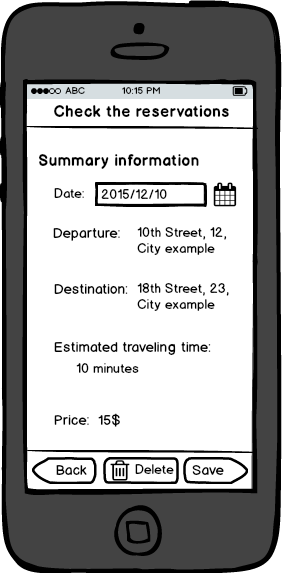
\includegraphics[height = 8 cm]{mockups/CheckReservations_MA_2}
		\caption[Modify reservations into mobile application.]{The page where a reservation can be modified or be cancelled into mobile application.}
		\label{UI:reservationMA2}
	\end{minipage}
\end{figure}

In \gls{ws} the same operations can be performed into the same page, displayed in figure \ref{UI:reservationWS}.

\begin{figure}[ht!]
	\centering
	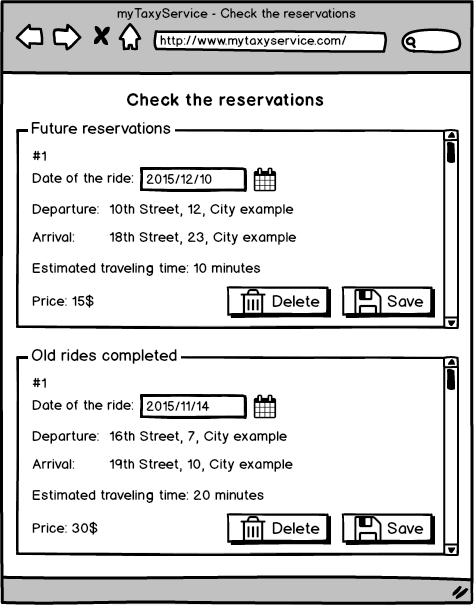
\includegraphics[height = 7.5 cm]{mockups/CheckReservations_WS}
	\caption[Check reservation into website.]{The check reservation page into page.}
	\label{UI:reservationWS}
\end{figure}

\clearpage

Finally, the user can received some alerts regarding, for instance, the assignment of the ride for which he asked for. The alerts can also be a general information, related to some problems of the service or to a strike.\\
The corresponding screen for the \gls{ma} and the \gls{ws} are shown, respectively, in figures \ref{UI:alertsMA} and \ref{UI:alertsWS}.

\begin{figure}[ht!]
	\centering
	\begin{minipage}[t]{0.4\textwidth}
		\centering
		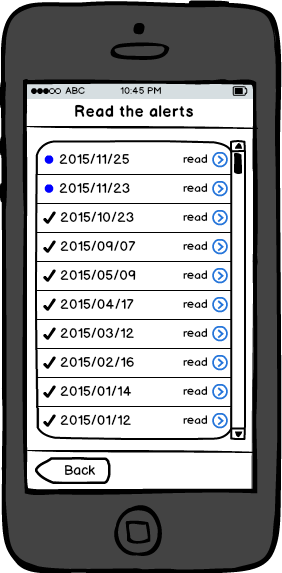
\includegraphics[height = 7 cm]{mockups/ReadAlerts_MA}
		\caption[Read the alerts into mobile application.]{The alerts page into mobile application.}
		\label{UI:alertsMA}
	\end{minipage}
	\hspace{0.5 cm}
	\begin{minipage}[t]{0.40\linewidth}
		\centering
		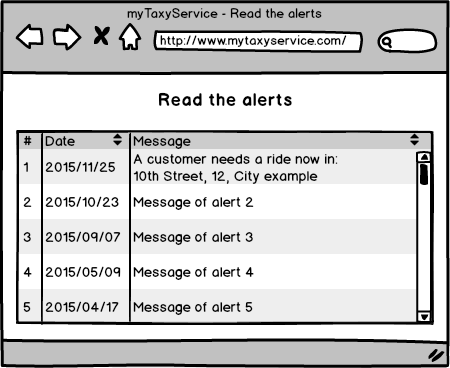
\includegraphics[width = \linewidth]{mockups/ReadAlerts_WS}
		\caption[Read the alerts into website.]{The alerts page into website.}
		\label{UI:alertsWS}
	\end{minipage}
\end{figure}

%End of chapter
\end{document}